\section{Experimental Results}
\label{sec:main_results}

We conduct comprehensive evaluation on FoldBench~\cite{xu2025benchmarking}, a standardized benchmark covering diverse biomolecular structure prediction tasks. We compare \texttt{SeedFold} against state-of-the-art methods including AlphaFold 3~\cite{abramson2024accurate}, Boltz-1~\cite{wohlwend2025boltz}, Protenix~\cite{bytedance2025protenix}\footnote{\texttt{https://github.com/bytedance/Protenix}, version 0.6.1.}, and Chai-1~\cite{chai2024chai}. The performance of AlphaFold 3, Boltz-1, Chai-1 are cited directly from FoldBench. 

\begin{table}[t]
    \centering
    \caption{Main results on FoldBench. Success rates are reported for interface tasks (DockQ $\geq 0.23$ for protein interfaces,  lRMSD $< 2$\AA~and lDDT-PLI $> 0.8$ for ligands). For all metrics, higher is better. The results of AlphaFold3, Boltz-1 and Chai-1 are retrieved from the FoldBench paper \cite{xu2025benchmarking}. We re-evaluated Protenix-0.5, a newer version than the one employed in FoldBench. For monomers, the underline symbol $\_$ denotes that results with higher precision are not provided in FoldBench.}
    \label{tab:main_results}
    \begin{tabular}{lcccccccc}
        \toprule
        \textbf{Model} & \makecell{\textbf{Monomer}\\\textbf{(lDDT)}} & \makecell{\textbf{Prot-Prot}\\\textbf{(DockQ)}} & \makecell{\textbf{Ab-Ag}\\\textbf{(DockQ)}} & \makecell{\textbf{Prot-Lig}\\\textbf{(SR\%)}} &
        \makecell{\textbf{Prot-RNA}\\\textbf{(DockQ\%)}} &
        \makecell{\textbf{Prot-DNA}\\\textbf{(DockQ\%)}} &
        \makecell{\textbf{DNA}\\\textbf{(lDDT)}} &
        \makecell{\textbf{RNA}\\\textbf{(lDDT)}}
        \\
        \midrule
        AlphaFold 3 & $0.88\_$ & $72.93\%$ & $47.90\%$ & $64.90\%$ & $62.32\%$ & $\mathbf{79.18\%}$ & $0.61\_$ & $\mathbf{0.53\_}$ \\
        Boltz-1 & $0.87\_$ & $68.25\%$ & $33.54\%$ & $55.04\%$ & $56.90\%$ & $70.97\%$ & $0.44\_$ & $0.34\_$ \\
        Chai-1 & $0.87\_$ & $68.53\%$ & $23.64\%$ & $51.23\%$ & $50.91\%$ & $69.97\%$ & $0.49\_$ & $0.46\_$\\
        Protenix-0.5 & $0.8773$ & $71.50\%$ & $41.00\%$ & $62.30\%$ & $50.70\%$ & $71.38\%$ & $\mathbf{0.6249}$ & $0.4930$\\
        \midrule
        \textbf{SeedFold} & $\mathbf{0.8889}$ & $74.03\%$ & $\mathbf{53.21}\%$ & $63.12\%$ & $\mathbf{65.31}\%$ & $72.60\%$ & $0.5897$ & $0.4990$ \\
        \textbf{SeedFold-Linear} & $0.8861$ & $\mathbf{74.14\%}$ & $46.91\%$ & $\mathbf{66.48\%}$ & $61.80\%$ & $76.00$ & $0.5965$ & $0.4610$ \\
        \bottomrule
    \end{tabular}
\end{table}
% \todoq{underline the second best result in the table?} -> yi: AF3 will have many underlines.


\subsection{Benchmark}

% \begin{table}[t]
%     \centering
%     \caption{Main results on FoldBench. Success rates are reported for interface tasks (DockQ $\geq 0.23$ for protein interfaces,  lRMSD ($< 2$\AA) and lDDT-PLI ($> 0.8$) for ligands). $\uparrow$ indicates higher is better.}
%     \label{tab:main_results}
%     \begin{tabular}{lcccc}
%         \toprule
%         \textbf{Model} & \makecell{\textbf{Monomer-Prot}\\\textbf{(lDDT$\uparrow$)}} & \makecell{\textbf{Prot-Prot}\\\textbf{(DockQ$\uparrow$)}} & \makecell{\textbf{Ab-Ag}\\\textbf{(DockQ$\uparrow$)}} & \makecell{\textbf{Prot-Lig}\\\textbf{(SR\%$\uparrow$)}} \\
%         \midrule
%         AlphaFold 3 & $0.8800$ & $70.29\%$ & $41.57\%$ & $61.78\%$ \\
%         Boltz-1 & $0.8707$ & $69.12\%$ & $31.38\%$ & $53.10\%$ \\
%         Protenix-0.5 & $0.8724$ & $67.52\%$ & $38.55\%$ & $55.49\%$ \\
%         \midrule
%         \textbf{SeedFold} & $\emph{0.8846}$ & $\mathbf{73.0\%}$ & $\mathbf{45.4\%}$ & $58.4\%$ \\
%         \textbf{SeedFold-Linear} & $\mathbf{0.8876}$ & $\emph{71.53\%}$ & $40.99\%$ & $\mathbf{63.29\%}$ \\
%         \bottomrule
%     \end{tabular}
% \end{table}


\paragraph{Experimental Setup}
FoldBench consists of $1,522$ biological assemblies spanning nine prediction tasks, with structures deposited after 2023-01-13. The benchmark includes: (i) \textbf{Monomers}: $334$ protein, $14$ RNA, and $15$ DNA monomers; (ii) \textbf{Interfaces}: $279$ protein-protein, $172$ antibody-antigen, $558$ protein-ligand, $70$ protein-RNA, $330$ protein-DNA, and $51$ protein-peptide interfaces. All targets are filtered for low homology to training sets to ensure fair evaluation. Following FoldBench, we adopt the $5\times5$ sampling strategy ($5$ random seeds $\times$ $5$ diffusion samples) with $10$ recycling steps. The best prediction is selected using the model's ranking score.


\begin{figure}[t]
    \centering
    \begin{minipage}[t]{0.32\textwidth}
        \centering
        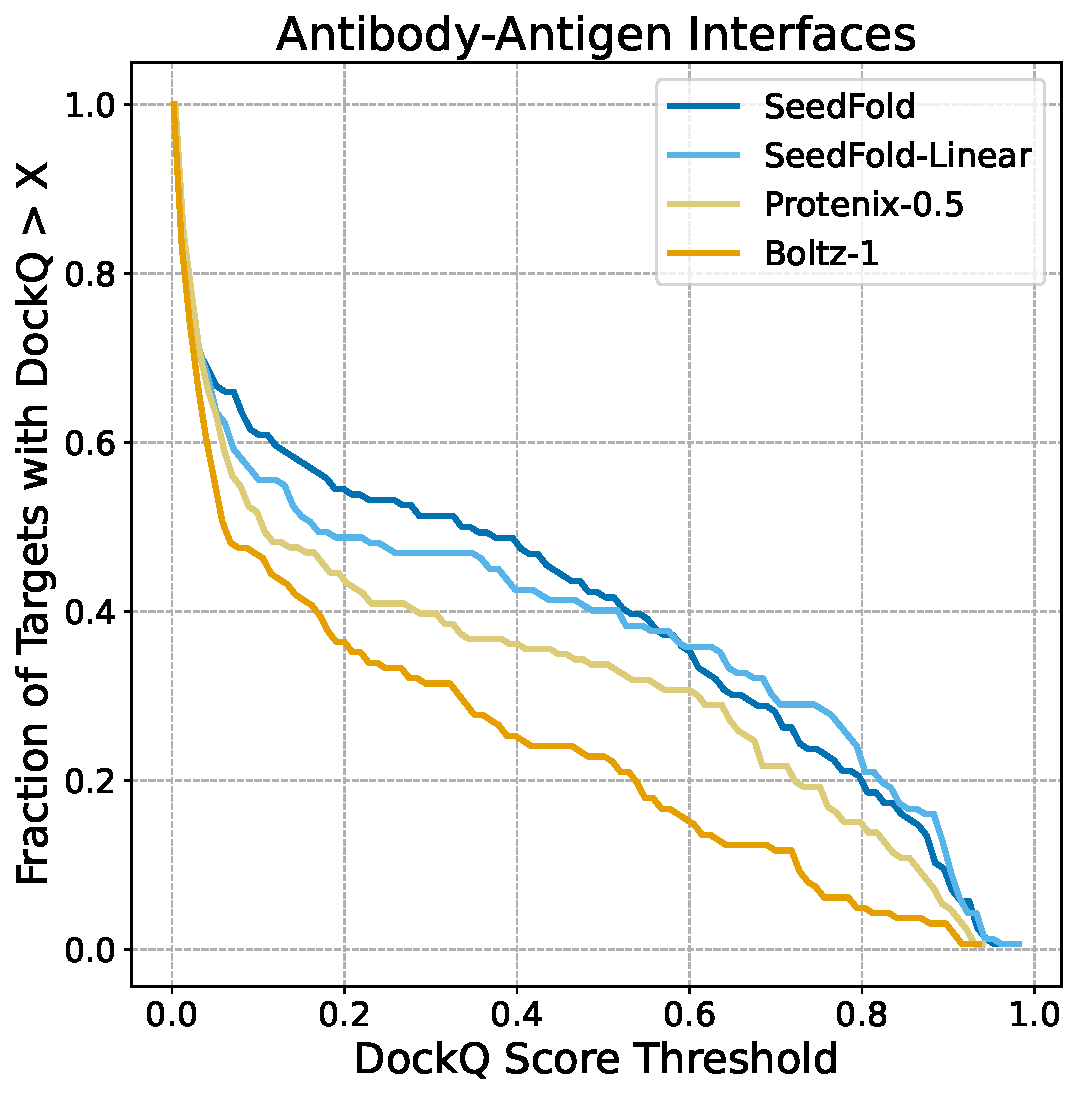
\includegraphics[width=\linewidth]{figures/interface_antibody_antigen_cumulative_dockq.pdf}
        % (a) Ab-Ag
    \end{minipage}
    \hfill
    \begin{minipage}[t]{0.32\textwidth}
        \centering
        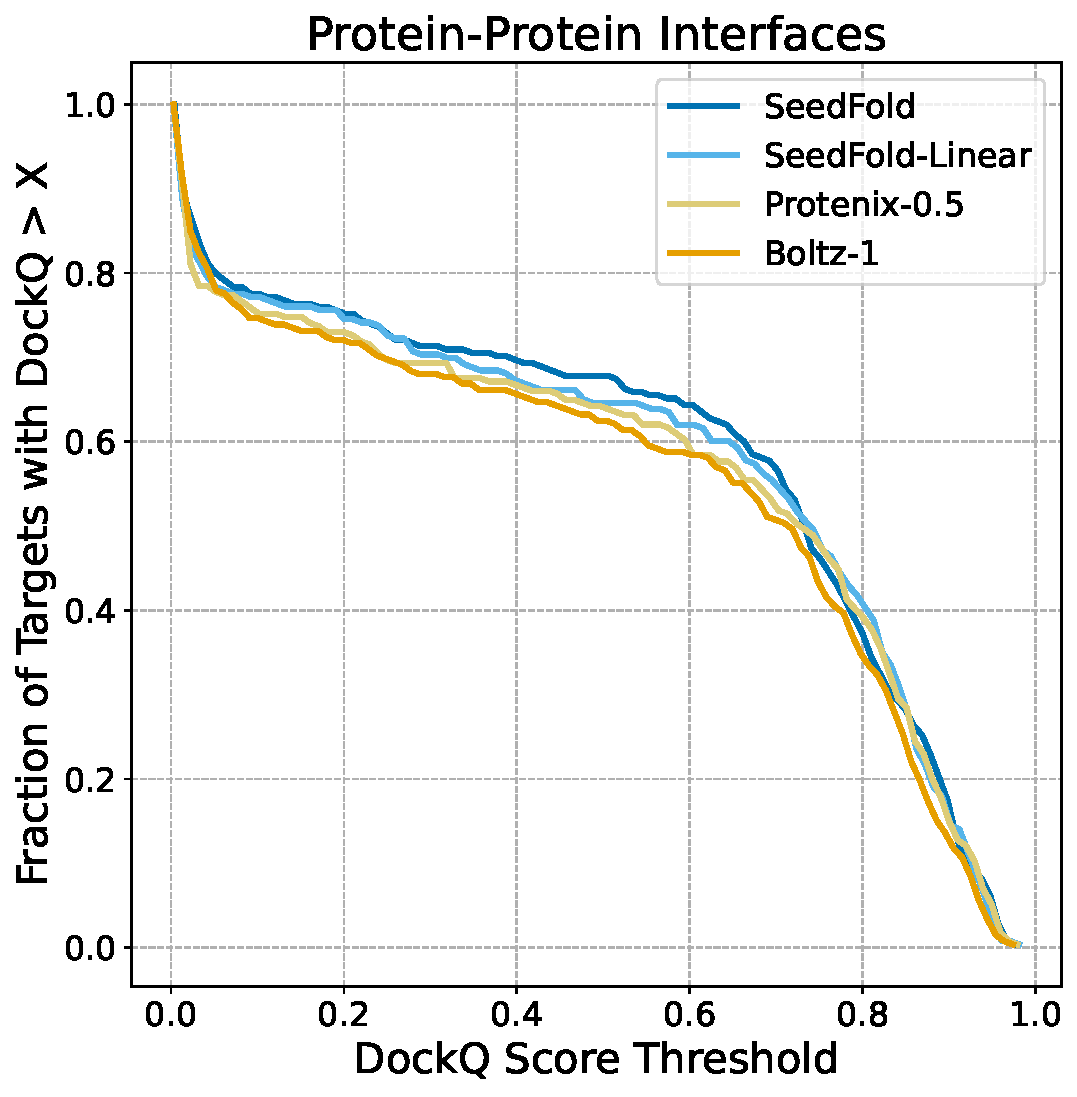
\includegraphics[width=\linewidth]{figures/interface_protein_protein_cumulative_dockq.pdf}
        % (b) Protein-Protein 
    \end{minipage}
    \hfill
    \begin{minipage}[t]{0.32\textwidth}
        \centering
        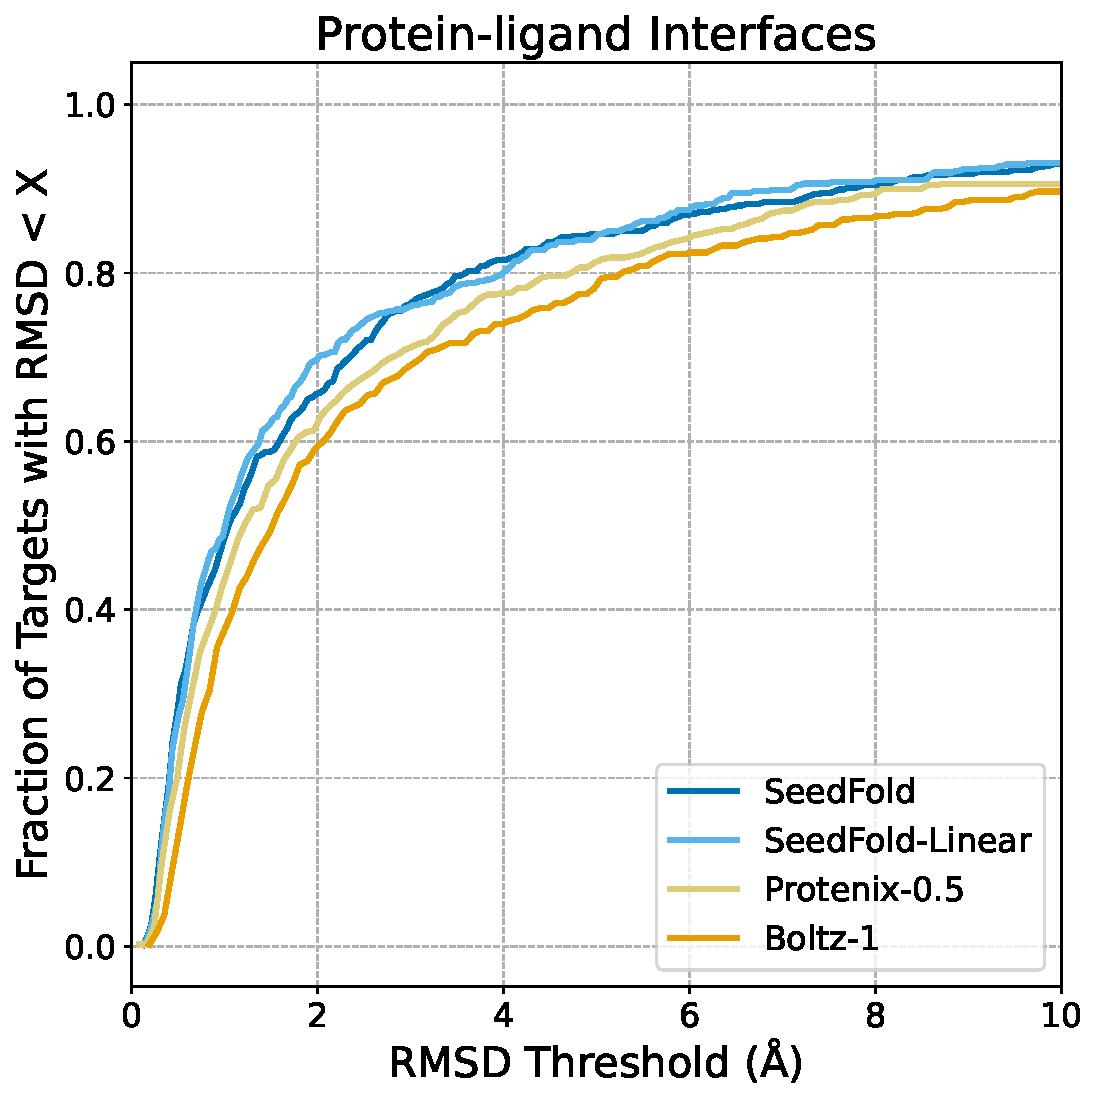
\includegraphics[width=\linewidth]{figures/interface_protein_ligand_cumulative_rmsd.pdf}
        % (c) Protein-Ligand
    \end{minipage}
    \caption{Cumulative distribution of interface prediction success rates across different modalities. We compare \texttt{SeedFold} and \texttt{SeedFold-Linear} against Boltz-1~\cite{wohlwend2025boltz} and Protenix-0.5~\cite{bytedance2025protenix}. Note that AlphaFold 3's detailed distribution metrics are not available due to license restrictions; their performance could be found in FoldBench~\cite{xu2025benchmarking}.}
    \label{fig:interface_distribution}
\end{figure}

% \paragraph{Protein Monomers}
% Table~\ref{tab:main_results} presents the main results on FoldBench. For protein monomers, \texttt{SeedFold} achieves an lDDT of $0.8889$, surpassing AlphaFold 3 ($0.88$) and outperforming Boltz-1 ($0.87$) and Protenix-0.5 ($0.8773$). \texttt{SeedFold-Linear} achieves a high lDDT of $0.8861$, demonstrating that linear attention does not compromise monomer prediction quality.


\begin{figure}[t]
    \centering
    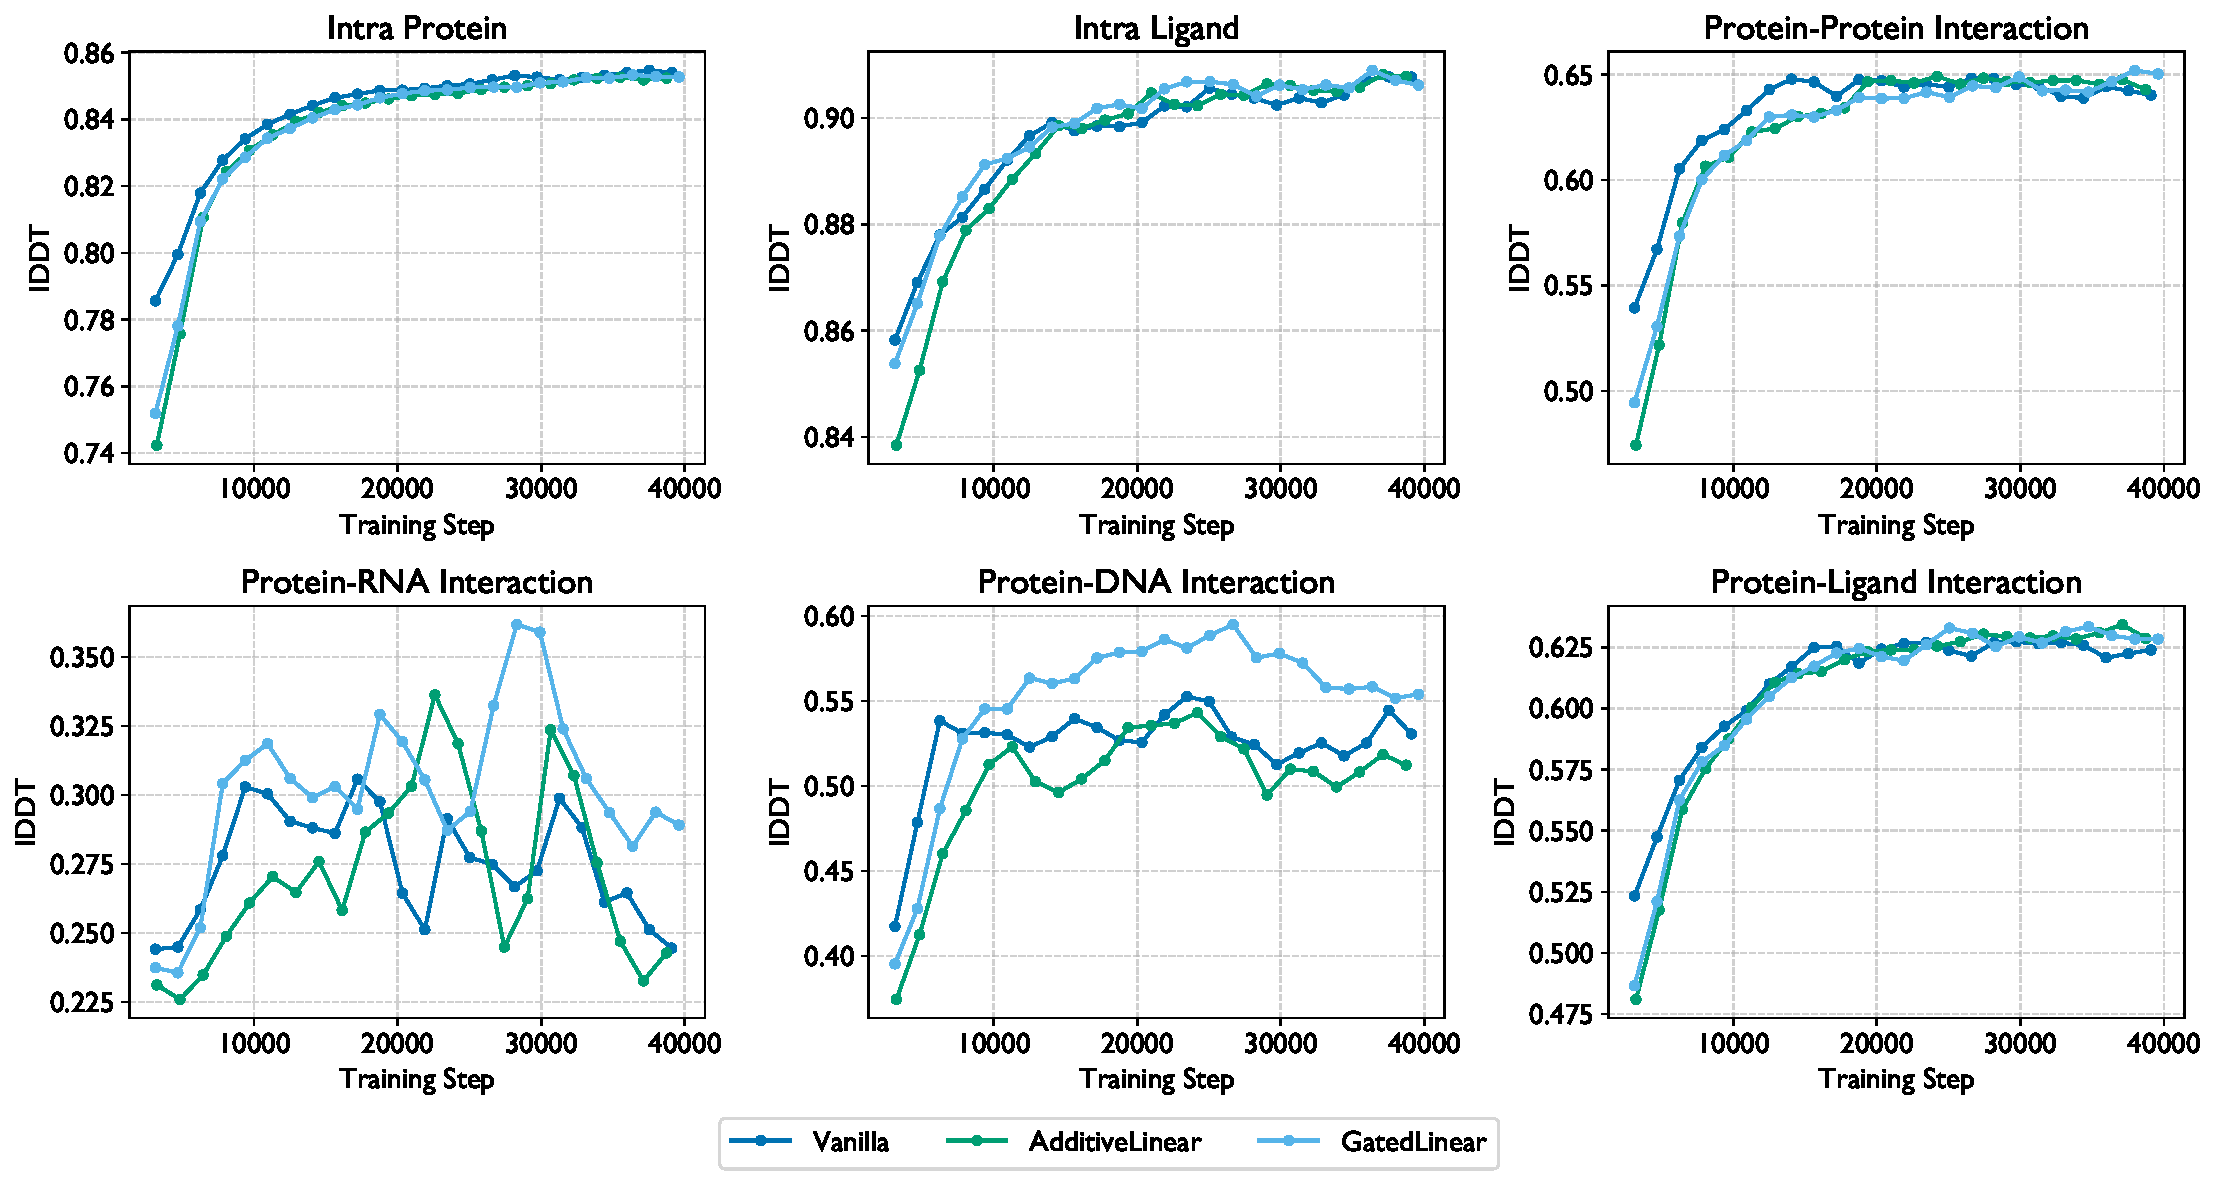
\includegraphics[width=1.0\linewidth]{figures/triatt_ablation.pdf}
    \caption{The validation scores across various metrics for different types of triangular attention are presented as follows. Linear triangular attention achieves on-par results on most metrics; moreover, in RNA/DNA-related tasks, \texttt{GatedLinearTriAtt} outperforms \texttt{AdditiveLinearTriAtt} and the standard attention mechanism.}
    \label{fig:triatt_ablation}
\end{figure}

% \paragraph{Protein-Protein Interfaces}
% For protein-protein interfaces, \texttt{SeedFold} achieves a DockQ success rate of $74.03\%$, significantly outperforming AlphaFold 3 ($72.93\%$), Boltz-1 ($68.25\%$), and Protenix-0.5 ($71.50\%$). \texttt{SeedFold-Linear} also demonstrates strong performance with $74.14\%$ success rate, exceeding AlphaFold 3.

% \paragraph{Antibody-Antigen Interfaces}
% Antibody-antigen prediction remains challenging for all methods. \texttt{SeedFold} achieves $53.21\%$ success rate, substantially outperforming AlphaFold 3 ($47.90\%$), Boltz-1 ($33.54\%$), and Protenix-0.5 ($41.00\%$). \texttt{SeedFold-Linear} achieves $46.91\%$, comparable to AlphaFold 3.

% \paragraph{Protein-Ligand Interactions}
% For protein-ligand docking, \texttt{SeedFold-Linear} achieves the best success rate of $66.48\%$, surpassing AlphaFold 3 ($64.90\%$) and significantly outperforming Boltz-1 ($55.04\%$) and Protenix-0.5 ($62.30\%$). The vanilla \texttt{SeedFold} achieves $63.12\%$, competitive with other open-source models.

% \paragraph{Protein-RNA and Protein-DNA Interfaces}
% For protein-RNA interfaces, \texttt{SeedFold} demonstrates state-of-the-art performance with a DockQ success rate of $65.31\%$, surpassing AlphaFold 3 ($62.32\%$). In protein-DNA interface prediction, \texttt{SeedFold-Linear} achieves a success rate of $76.00\%$, which is the best among open-source models and second only to AlphaFold 3 ($79.18\%$).

% \paragraph{RNA and DNA Monomers}
% For nucleic acid monomer prediction, our models demonstrate competitive performance. For DNA monomers, \texttt{SeedFold-Linear} (lDDT $0.5965$) and \texttt{SeedFold} (lDDT $0.5897$) are competitive. For RNA monomers, \texttt{SeedFold} achieves an lDDT of $0.4990$, outperforming most open-source models.

% \paragraph{Summary}
% The two variants exhibit different strengths. The vanilla \texttt{SeedFold} excels at protein monomers, antibody-antigen, and protein-RNA interfaces. The \texttt{SeedFold-Linear} model shows superior performance on protein-protein, protein-ligand, and protein-DNA interfaces. Both variants consistently outperform existing open-source models across most evaluated tasks, demonstrating the effectiveness of our approach.

\paragraph{Overall Peformance} As detailed in Table~\ref{tab:main_results}, our models demonstrate state-of-the-art or highly competitive performance across the majority of FoldBench tasks. The vanilla \texttt{SeedFold} model establishes new benchmarks in protein monomer prediction (lDDT $0.8889$), antibody-antigen interfaces ($53.21\%$ DockQ), and protein-RNA interfaces ($65.31\%$ DockQ), notably outperforming AlphaFold 3. Concurrently, the \texttt{SeedFold-Linear} variant shows its strength by leading in protein-ligand prediction ($66.48\%$ success rate) and protein-protein interfaces ($74.14\%$ DockQ). In the remaining tasks, including protein-DNA and nucleic acid monomer prediction, both models deliver strong results that are competitive with AlphaFold 3 and consistently surpass other open-source methods. Collectively, these results validate that our width-scaling strategy effectively enhances model capacity and that the linear triangular attention offers a computationally efficient yet powerful alternative to standard attention mechanisms.


\paragraph{Interface Prediction}
To further dissect the performance on key interface prediction tasks, we present the cumulative distribution of success rates in Figure~\ref{fig:interface_distribution}. These plots illustrate the fraction of targets achieving a quality score above a given threshold, offering a more granular view than summary metrics alone. For antibody-antigen interfaces, \texttt{SeedFold} demonstrates a commanding lead over all other models across the entire DockQ score range, indicating its superior accuracy and reliability for this challenging task. In protein-protein interface prediction, while all models perform competitively, both \texttt{SeedFold} and \texttt{SeedFold-Linear} maintain a consistent advantage over Protenix-0.5 and Boltz-1. For protein-ligand interfaces, our models again show a clear superiority, with \texttt{SeedFold-Linear} achieving the best performance. These detailed distributions underscore the significant improvements, providing more robust and accurate predictions across critical interface modeling domains.



% \subsection{Scaling Analysis}

% To understand the effect of model scaling, we compare models with different \texttt{Pairformer} widths trained under the same protocol.

% \paragraph{Training Set Fitting}
% We randomly sample $512$ cases from the training set to analyze fitting quality. As shown in Figure~\ref{fig:scaling_train}, larger models achieve consistently better fitting across all modalities:
% \begin{itemize}
%     \item The \texttt{Pairformer}'s distance prediction accuracy improves with increased width.
%     \item The diffusion module generates higher-quality structures with richer trunk representations.
% \end{itemize}

% \paragraph{Validation Performance}
% Table~\ref{tab:scaling_results} shows that validation performance follows the same trend as training, indicating effective generalization rather than overfitting.

% \begin{table}[h]
%     \centering
%     \caption{Effect of model scaling on FoldBench validation performance.}
%     \label{tab:scaling_results}
%     \begin{tabular}{lcccc}
%         \toprule
%         \textbf{Width} & \textbf{Protein (LDDT)} & \textbf{Prot-Prot (DockQ)} & \textbf{Prot-Lig (SR\%)} & \textbf{Train Speed} \\
%         \midrule
%         128 (Base) & -- & -- & -- & 3.2 iter/s \\
%         256 & -- & -- & -- & -- iter/s \\
%         384 & -- & -- & -- & -- iter/s \\
%         \bottomrule
%     \end{tabular}
% \end{table}



\subsection{Ablation Studies}

We conduct ablation studies to understand the contribution of each component.

% \paragraph{Attention Mechanism}
% Figure~\ref{fig:triatt_ablation} compares our linear triangular attention variants against standard triangular attention. While both of the two linear variants can yield similar results across most metrics, the \texttt{GatedLinearTriAtt} performs better on DNA/RNA-related tasks. A key difference between \texttt{GatedLinearTriAtt} and \texttt{AdditiveLinearTriAtt} lies in the choice of operation between $\mathbf{QK}^T$ and $\mathbf{B}$. We selected \texttt{GatedLinearTriAtt} because the multiplication operation offers greater expressive capacity, whereas the addition operation may result in a low-rank attention matrix~\cite{fan2025breaking}. Nevertheless, \texttt{AdditiveLinearTriAtt} can still achieve performance similar to that of the gated version. Figure~\ref{fig:lin_interface_distribution} shows that the gated variant can better capture the correlation for antibody-antigen and protein-ligand interfaces.


\paragraph{Attention Mechanism}
To validate our design choices of different attention mechanisms, we conducted a comprehensive ablation study comparing three attention variants: (i) the standard softmax attention (\texttt{VanillaTriAtt}), (ii) a linear version with an additive feature map (\texttt{AdditiveLinearTriAtt}), and (iii) our proposed gated version (\texttt{GatedLinearTriAtt}). As shown in Figure~\ref{fig:triatt_ablation}, the validation curves reveal that both linear attention variants achieve performance on par with the vanilla attention across most prediction tasks, including intra-protein and protein-protein interactions. Notably, for tasks involving nucleic acids (protein-RNA and protein-DNA), the \texttt{GatedLinearTriAtt} variant demonstrates a clear and consistent advantage over both the additive version and the standard softmax attention, indicating its enhanced capability in handling diverse molecular types.

To further refine our choice, we performed a detailed head-to-head comparison between \texttt{GatedLinearTriAtt} and \texttt{AdditiveLinearTriAtt} on key interface prediction tasks (Figure~\ref{fig:lin_interface_distribution}). The cumulative distribution plots show that \texttt{GatedLinearTriAtt} holds a slight but consistent edge in antibody-antigen and protein-ligand interface predictions. Given its superior performance on nucleic acid and antibody tasks without compromising efficacy elsewhere, we selected \texttt{GatedLinearTriAtt} as the default configuration for our \texttt{SeedFold-Linear} model, confirming it as a powerful and efficient alternative to standard attention.



\paragraph{Monomer Distillation}
Monomer distillation data is a key component of our training set, designed to ground the model's understanding of fundamental protein geometry. To verify its importance throughout the entire training process, we conducted an ablation study. Starting from a checkpoint at $47,612$ steps (trained on the full dataset), we continued training under two conditions: one with the complete dataset, and another where the monomer distillation data was removed. Figure~\ref{fig:distill} (in Appendix~\ref{appendix:data}) shows that removing the distillation data leads to a significant and immediate degradation in intra-protein structure prediction accuracy. While the impact on direct interface metrics appears less pronounced in the short term, maintaining the model's fundamental ability to accurately fold single protein chains is critical for its overall predictive power. This finding underscores the importance of including monomer distillation data throughout the entire training process to prevent knowledge decay and ensure the model's robustness.

